\documentclass[lettersize,journal, one-column]{IEEEtran}
%\documentclass[journal, a4paper, onecolumn, draftcls]{IEEEtran}
\usepackage{amsmath,amsfonts}
\usepackage{algorithmic}
\usepackage{algorithm}
\usepackage{array}
\usepackage{subcaption}
\captionsetup{compatibility=false}
\usepackage{textcomp}
\usepackage{stfloats}
\usepackage{url}
\usepackage{verbatim}
\usepackage{graphicx}
\usepackage{cite}
\usepackage{varwidth}
\usepackage{hhline}
\usepackage{multirow}
\usepackage[inline]{enumitem}

\begin{document}

\title{Lightpath Length and Launch Power Estimation with Machine Learning}

\author{Shayan Hajipour}


\maketitle

\begin{abstract}
Lightpath distance between transmitter and constellation profile observation points and launch power are predicted with linear regression and support vector machine.
\end{abstract}

\section{Introduction}
\label{section:introduction}
Digital twins (DTs) with proper abstractions could be used for deriving insights, diagnosis, planning, and carrying out drills on complex systems.
An analytical DT called GNPy is already developed for signal propagation in optical networks~\cite{gnpy}.
However, sometimes analytical DTs are hard to create.
Machine learning (ML) approach is the algorithmically simple candidate for building DTs with minimal knowldege in subject matter.

An ML-based DT could be used to estimate lightpath (LP) attributes (e.g., launch power and distance) given In-Phase and Quadrature (IQ) optical constellation diagrams.
For example, LP launch power estimation could be used to dignose potential discrepancies between planned, telemetry, and actual launch power. 
Such attribute estimations could be performed at the pass through observation points via optical spectrum analyzers to give a better resolution of the LP status as well as receiver site~\cite{9761942}.
After discrepancy detection, the adopted remediatory measures could be initiated.

In this report, we estimate and launch power and the distance between transmitter and observation point of lucid lightpaths.

\section{Dataset}
\label{section:dataset}
The datasets are collected by numerical simulations of two scenario configurations:
\begin{enumerate}
    \item \textit{Single link scenario}, where LPs travel up to 25 spans deployed between the transmitter and receiver.
    The observation point is the receiver, where the IQ constellation profile consisting of 2048 symbol samples are scanned for each datapoint.
    The number of spans and the length of the first span are the labeled variables of the dataset.
    The length of the first span could be 80 km, 60 km, or 40 km, which are called \textit{optimal}, \textit{sub-optimal}, and \textit{degradation} modes, respectively.
    The length of other spans is 80 km.
    The total number of  2250 scans (datapoints) of IQ constellation profile are collected.
    Each datapoint consists of 2048$\times$2+1+1 columns that represent in-phase and quadrature components of symbol samples, the distance between the transmitter and the observation point, and datpoint mode.
    \item \textit{multiple links scenario}, where LPs travel 5 reconfigurable optical add-drop multiplexers (ROADMs) and 4 equal links.
    The number and length of spans in each link, launch power, and the observation point are the labeled variables of the dataset.
    The observation point candidates are ingress and egress ports of ROADMs, where the IQ constellation profile consisting of 8192 symbol samples are scanned for each datapoint.
    The total number of 800 scans (datapoints) of IQ constellation profile are collected.
    Each datapoint consists of 8192$\times$2+1+1+1 columns that represent in-phase and quadrature components of symbol samples, the distance between the transmitter and the observation point, the ROADM side of the observation point, and the launch power.
    The ROADM side could be ingress or egress, which is represented with a binary.
    The launch power is wether 1 or 2 dBm, which is also represented with a binary.
\end{enumerate}
The data generation simulation configurations are further elaborated in~\cite{data146_2022}.

\section{Machine Learning Models}
\label{section:ml_models}
We estimate the distance between the transmitter and the observation point in the single link scenario.
We also classifiy the launch power in the multiple links scenario since it is the lightpath configuration attribute and could be vulnerable to potential misconfiguration.
The ML pipeline for distance regression and launch power classification is shown in Fig.~\ref{figure:models}.
\begin{figure}
	\centering
    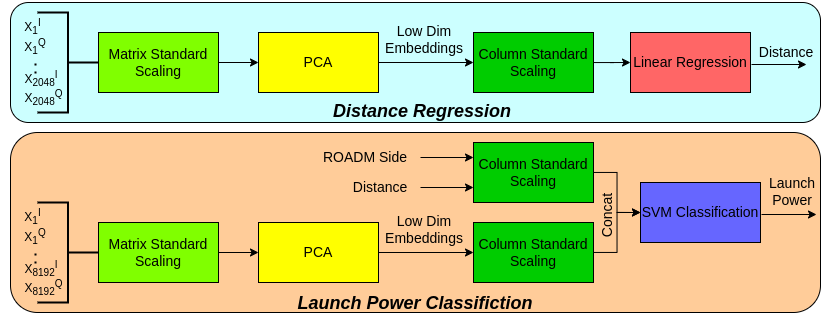
\includegraphics[width=\columnwidth]{figures/models.png}
    \caption{Lightpath attribute estimation pipelines}
	\label{figure:models}
\end{figure}
The IQ constellation profile is compressed with the principal component analysis (PCA) method.
PCA projects the oiginal data to low dim directions, which maximize the variance.
Before PCA, the data is scaled by a custom standard scaler that operates with $\frac{(\textbf{D}-\mu)}{\sigma}$, where $\textbf{D}$, $\mu$, and $\sigma$ are the IQ constellation profile, mean, and standard deviation of all columns of $\textbf{D}$.
A linear regression model estimates the distance for the single link scenario after another standard scaling across columns of low dimensional embeddings resulted from PCA.
The column standard scaler operates with $\frac{\textbf{D - M}}{\mathbf{\Sigma}}$, where $\textbf{D}$, $\textbf{M}$, and $\mathbf{\Sigma}$ are the IQ constellation profile, mean vector, and standard deviation vector of each column of $\textbf{D}$.
For launch power classification, the ROADM side and distance data are concatenated with the PCA embeddings after standard scaling across columns.
Then, a support vector machine (SVM) classification model classifies the launch power.

\section{Results}
\label{section:results}




\section{Conclusion}
\label{section:conclusion}


\begin{thebibliography}{1}
\bibliographystyle{IEEEtran}

\bibitem{gnpy}Project, T. GNPy: Optical Route Planning and DWDM Network Optimization. {\em GitHub Repository}. (2023), https://github.com/Telecominfraproject/oopt-gnpy

\bibitem{9761942}Ruiz, M., Sequeira, D. \& Velasco, L. Deep learning-based real-time analysis of lightpath optical constellations [Invited]. {\em Journal Of Optical Communications And Networking}. \textbf{14}, C70-C81 (2022)

\bibitem{data146_2022}Ruiz Ramírez, M., Velasco Esteban, L. \& Sequeira, D. Optical Constellation Analysis (OCATA). (CORA.Repositori de Dades de Recerca,2022), https://doi.org/10.34810/data146





\end{thebibliography}
\end{document}


